\chapter{Column Stores}
\textbf{Row Store:}
\begin{itemize}
    \item Data are stored in tables and on disk
    \item Stored consecutively
    \item Used in most RDBMs
\end{itemize}
\textbf{Column Store:}
\begin{itemize}
    \item Column oriented relational database
    \item Data are stored in tables but on disk
    \item Stored consecutively
\end{itemize}
Column store work very well for certain queries type like queries that can be executed on compressed data, indeed columns stores have the advantage of both a \textit{compact storage} as well as \textit{efficient query execution}.

\section{Column-Wise Storage}
We take up our tiny library example to illustrate the differences:
\begin{figure}[!hbp]
    \centering
    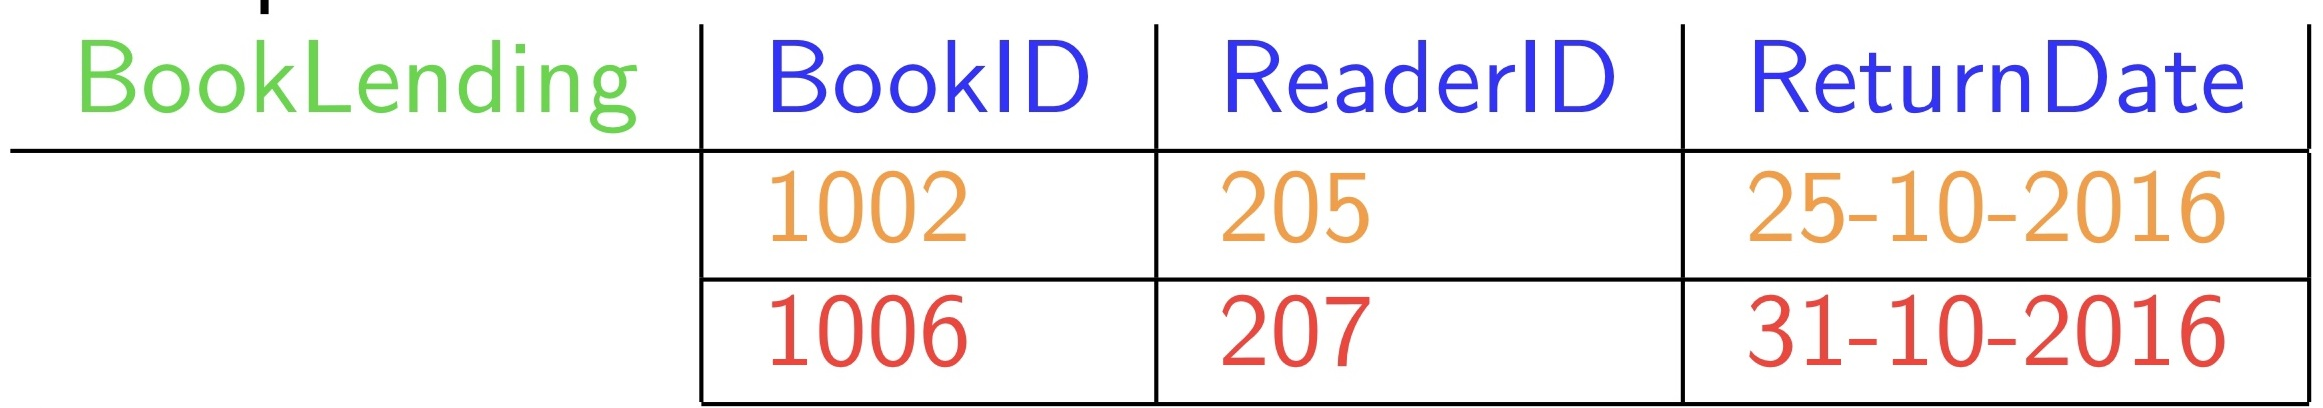
\includegraphics[width=0.60\linewidth]{images/AdvancedDataManagment/column_stores/library_example.jpeg}
    \caption{BookLending example}
\end{figure}

Storage order in row store:

\centerline{\textcolor{orange}{1002, 205, 25-10-2016}, \textcolor{red}{1006, 207, 31-10-2016}}

Storage order in column store:

\centerline{
\textcolor{orange}{1002}, \textcolor{red}{1006},
\textcolor{orange}{205}, \textcolor{red}{207},
\textcolor{orange}{25-10-2016}, \textcolor{red}{31-10-2016}
}
\textbf{Advantages} of column stores are for example:
\begin{itemize}
    \item \textbf{Buffer management:} only columns (attributes) that are needed are read from disk into main memory, because a single memory page ideally contains all values of a column.
    \begin{itemize}
        \item In row stores memory page might contain also other attributes, so data is fetched unnecessarily
    \end{itemize}
    \item \textbf{Homogeneity:} values in a column have the same type. This is why they can be compressed better when stored consecutively.
    \begin{itemize}
        \item In row stores values from different attribute domains are mixed in a row, so compression is not as good
    \end{itemize}
    \item \textbf{Data locality:} iterating or aggregating over values in a column can be done quickly.
    \begin{itemize}
        \item In row stores values have to be read and picked out from different tuples
    \end{itemize}
    \item \textbf{Column insertion:} adding new columns to a table is easy because they just can be appended to the existing ones
    \begin{itemize}
        \item  In row store, storage reorganization it necessary to append a new column value to each tuple
    \end{itemize}
\end{itemize}

\textbf{Disadvantages} of column stores are:
\begin{itemize}
    \item \textbf{Tuple reconstruction:} combining values from several columns is costly because “tuple reconstruction” has to be performed
    \begin{itemize}
        \item In row store, tuple reconstruction is not necessary because values of a tuple are stored consecutively
    \end{itemize}
    \item \textbf{Tuple insertion:} inserting a new tuple is costly
    \begin{itemize}
        \item In row store, the new tuple is appended to the existing ones and the new values are stored consecutively
    \end{itemize}
\end{itemize}

\subsection{Column Compression}
\begin{itemize}
    \item Values in a column range over the same attribute domain; that is, the have the same data type.
    \item Columns may contain lots of repetitions of individual values or sequences of values.
    \item These are two reasons why compression can be more effective on columns.
    \item Storage space needed in a column store may be less than storage space needed in a row store with the same data.
\end{itemize}
\newpage
 Having said that we can introduce five option for column data compression: 
\begin{itemize}
    \item \textbf{Run-length encoding:}
    \begin{itemize}
        \item The run-length of a value denotes how many repetitions of the value are stored consecutively
        \item We will store the value together with its starting row and its run-length
        \item This encoding is most efficient for long runs of repetitive values
    \end{itemize}
    \begin{figure}[!hbp]
        \centering
        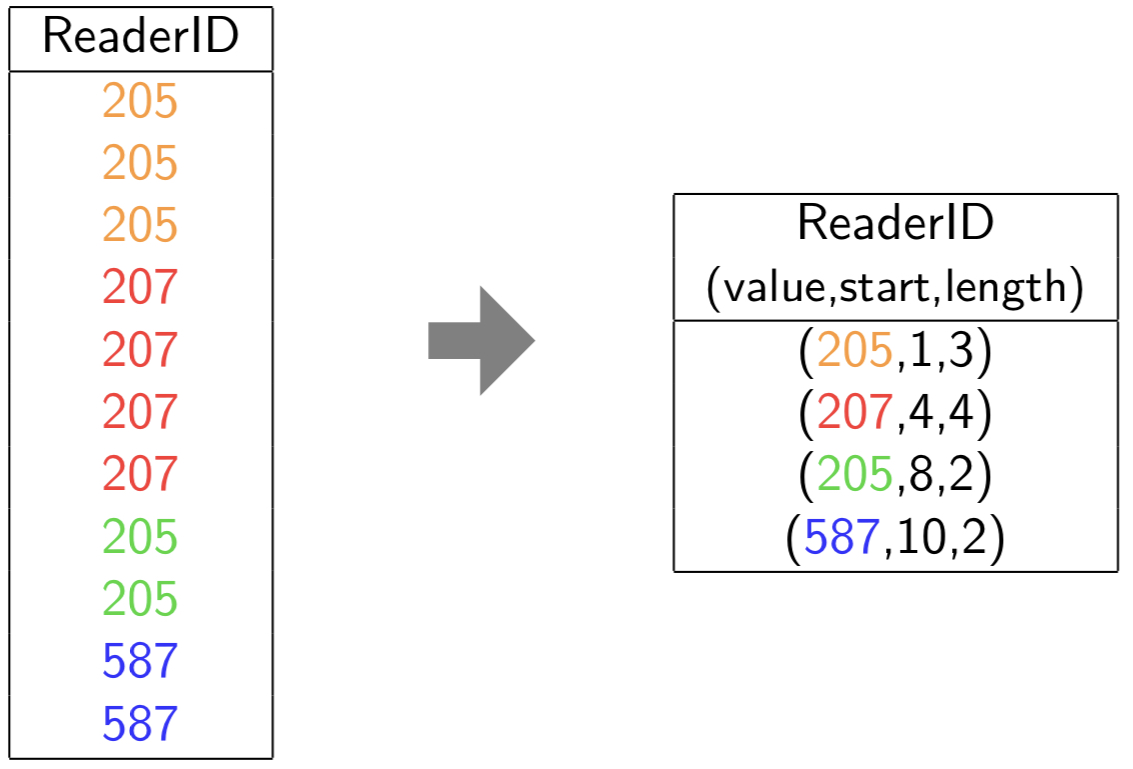
\includegraphics[width=0.60\linewidth]{images/AdvancedDataManagment/column_stores/run-length_encoding.jpeg}
        \caption{Run-length encoding example}
    \end{figure}
        
    
    \item \textbf{Bit-vector encoding:} 
    \begin{itemize}
        \item For each value in the column we create a bit vector with one bit for each row
        \item In each vector cell if the value is 1, it means the presence of the value in the column
        \item This encoding is most efficient for relatively few distinct values and hence relatively few bit vectors
    \end{itemize}
    
    
    \begin{figure}[!hbp]
        \centering
        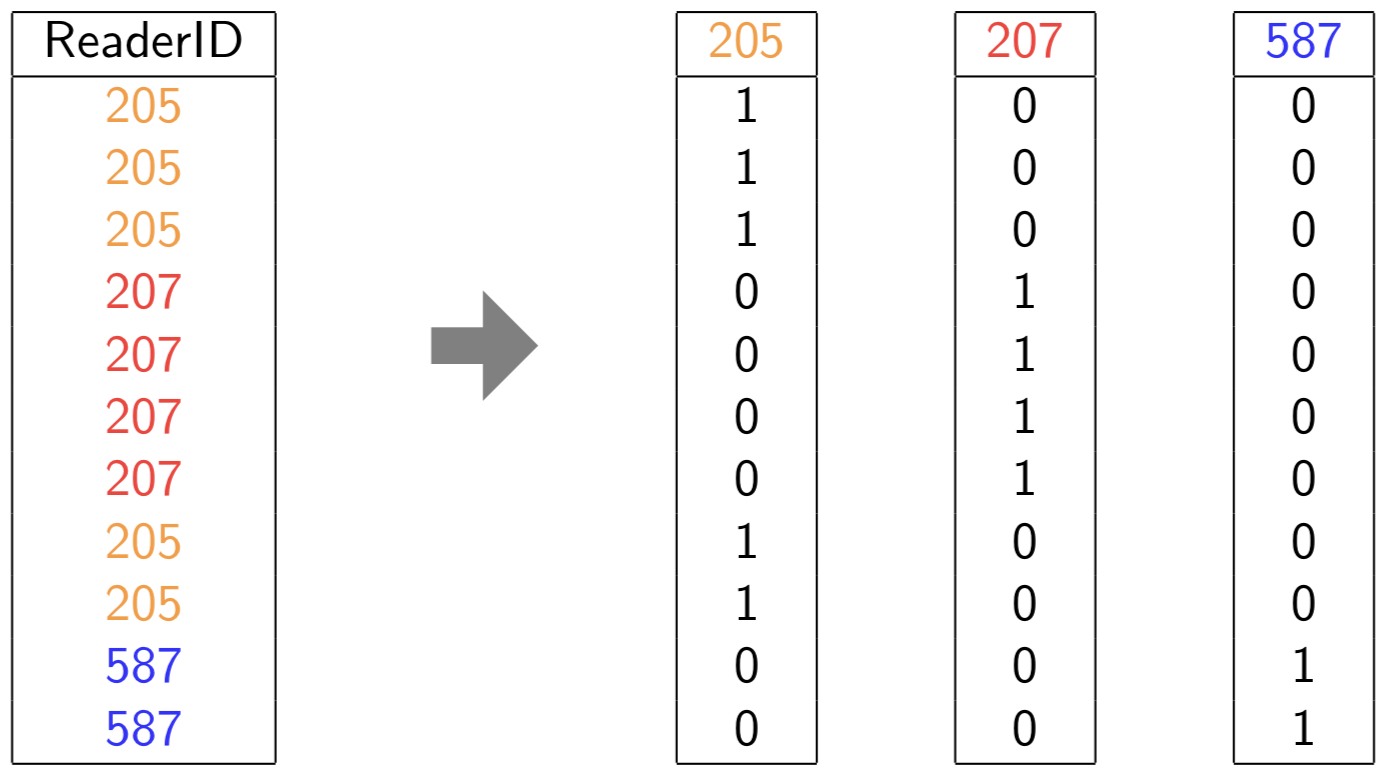
\includegraphics[width=0.60\linewidth]{images/AdvancedDataManagment/column_stores/bit_vector_encoding.jpeg}
        \caption{Bit vector encoding example}
    \end{figure}
    
    \newpage
    \item \textbf{Dictionary encoding:} 
    \begin{itemize}
        \item We replace long values by shorter placeholders and maintain a dictionary to map the placeholders back to the original values
        \begin{figure}[!hbp]
            \centering
            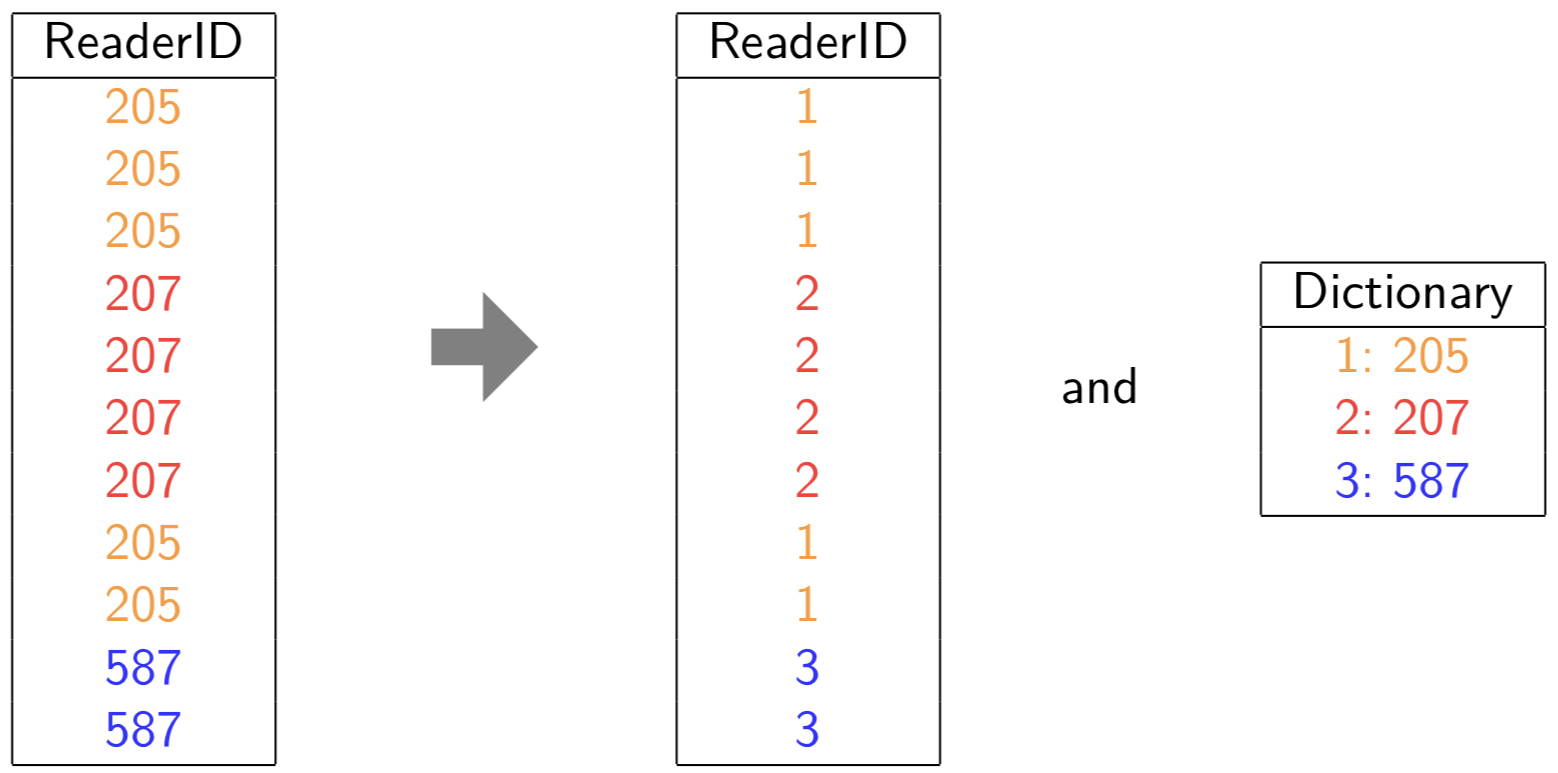
\includegraphics[width=0.50\linewidth]{images/AdvancedDataManagment/column_stores/dictionary_encoding.jpeg}
            \caption{Dictionary encoding example}
        \end{figure}
        \item In some cases, we could not only create a dictionary for single values but even for frequent sequences of values
        \begin{figure}[!hbp]
            \centering
            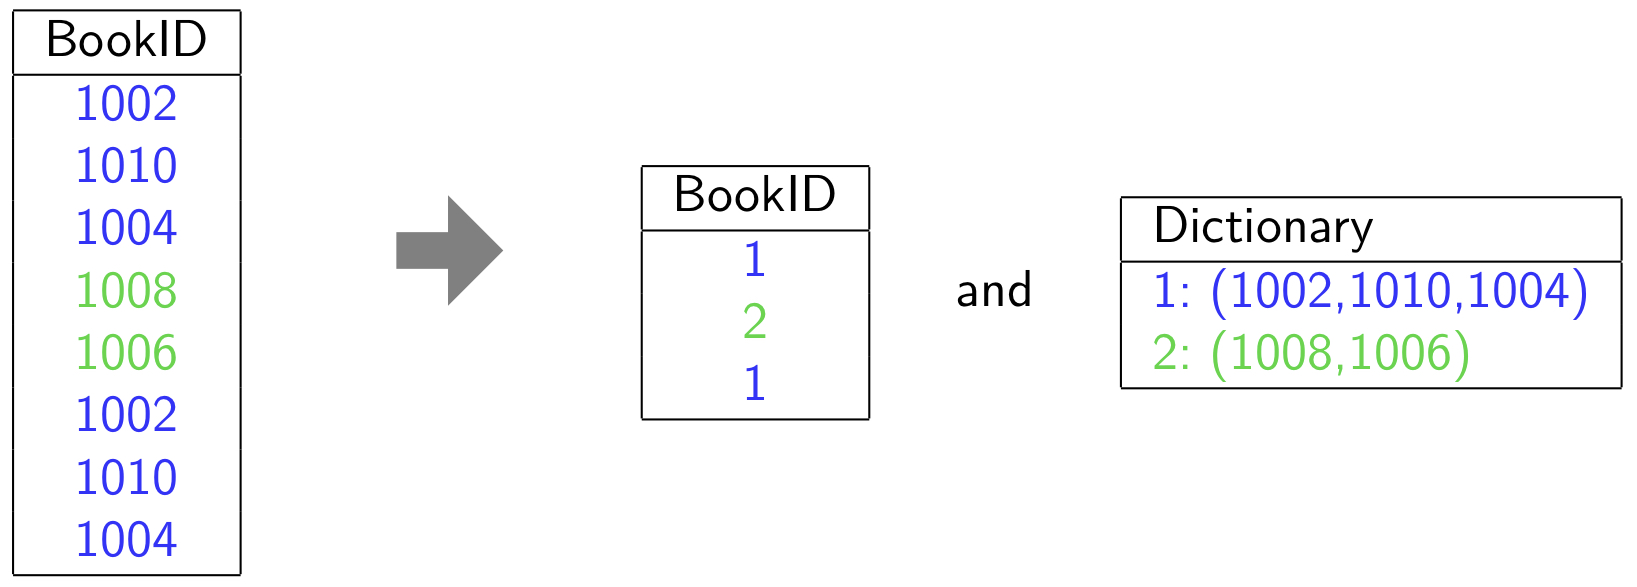
\includegraphics[width=0.40\linewidth]{images/AdvancedDataManagment/column_stores/dictionary_encoding_sequence.jpeg}
            \caption{Dictionary sequence encoding example}
        \end{figure}
    \end{itemize}
    
    
    \item \textbf{Frame of reference encoding:}
    \begin{itemize}
        \item For the range of values stored in a column, one value that lies in the middle of this range is chosen as the reference value
        \item For all other values we only store the off-set from the reference value, (smaller than the original value)
        \item \(3\) bit to store all. Interval \((-4, 4)\) so 2 bit plus the sign bit
    \end{itemize}
    
    
    \begin{figure}[!hbp]
        \centering
        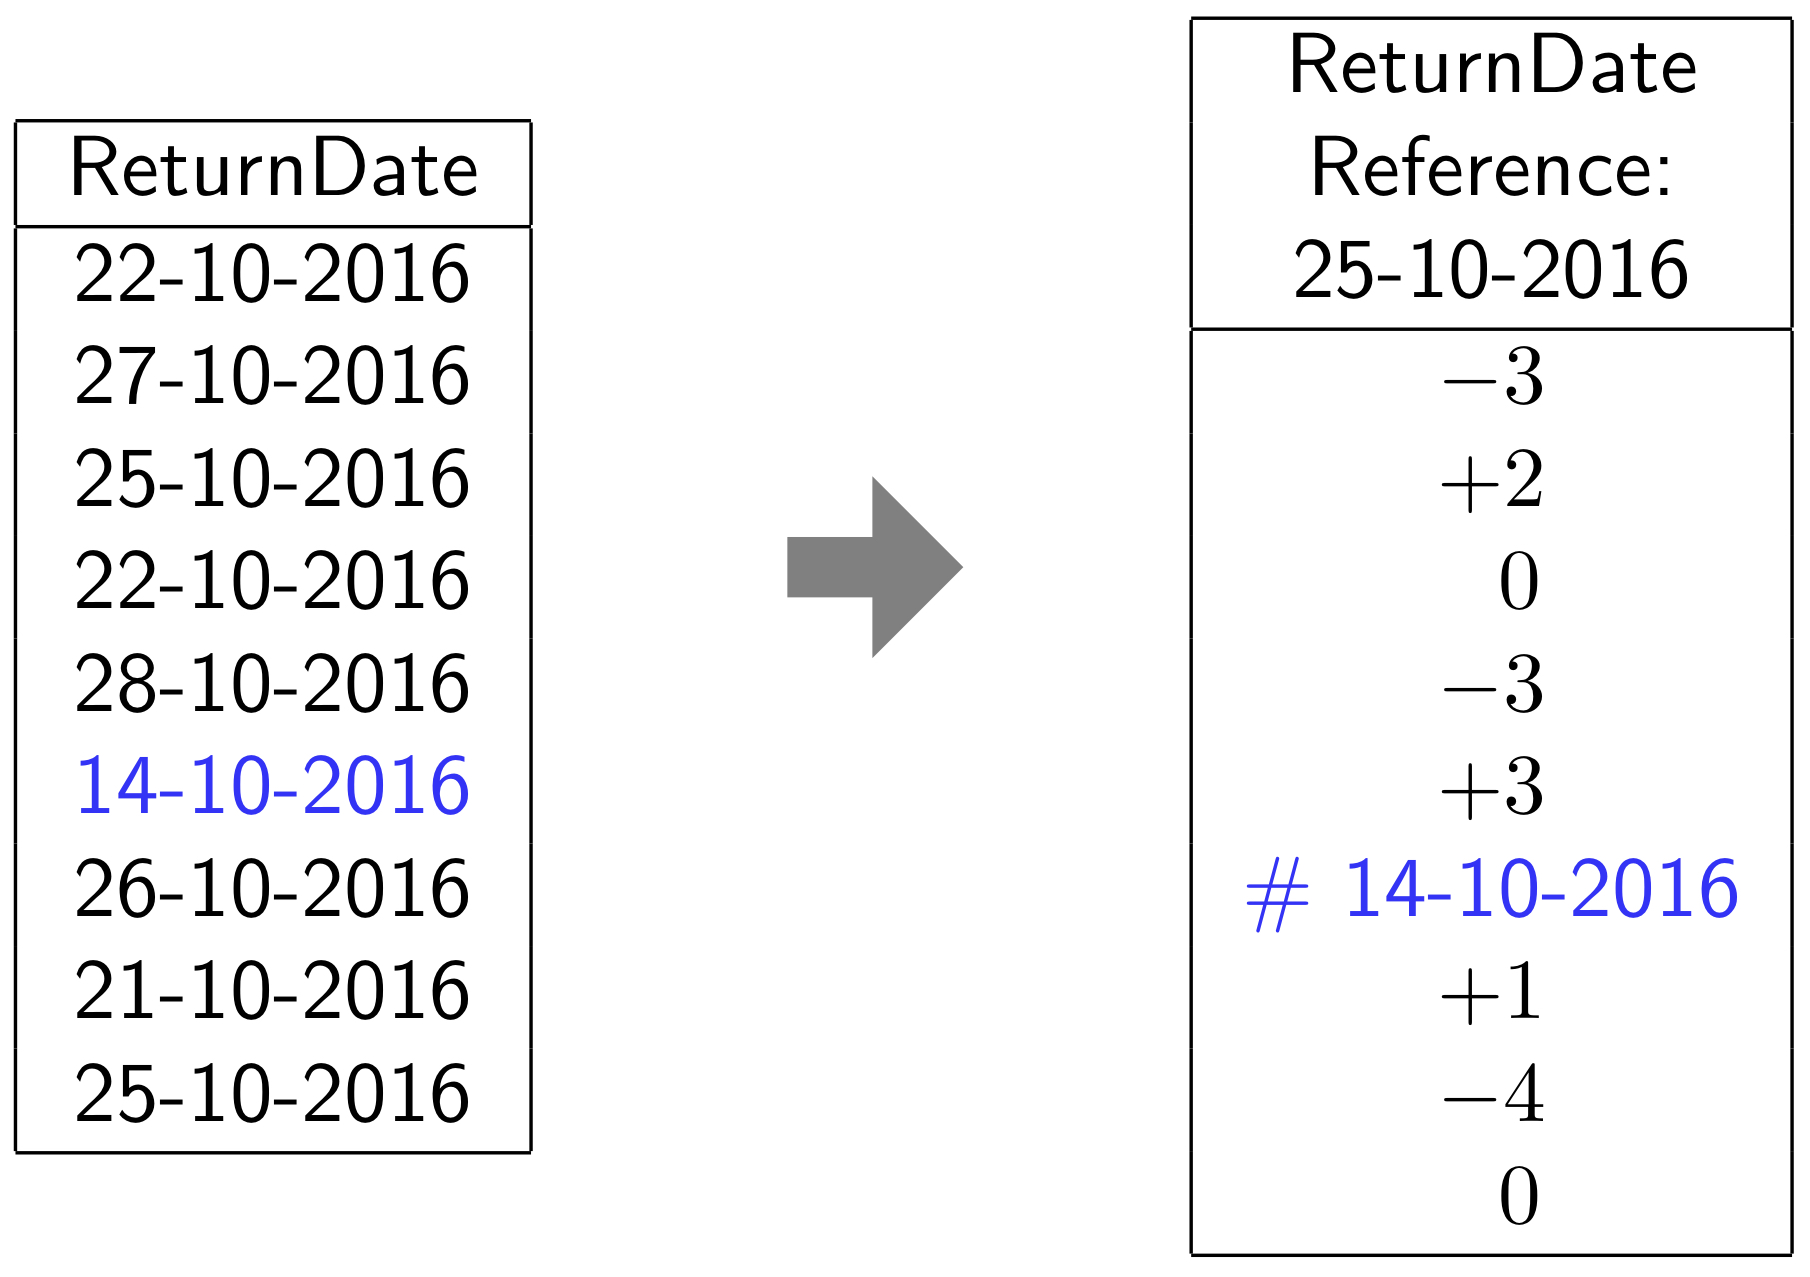
\includegraphics[width=0.60\linewidth]{images/AdvancedDataManagment/column_stores/frame_reference_encoding.jpeg}
        \caption{Frame reference encoding example}
    \end{figure}
    
    
    \item \textbf{Differential encoding:}
    \begin{itemize}
        \item An offset is stored instead of the entire value
        \item The offset is the difference between the value itself and the value in the preceding row
        \item Again the offset should not exceed a fixed size
        \item As soon as the offset gets too large, the current value is stored as an \textit{exception}
        \item This encoding is only applicable to numerical data
        \item It works best if data are stored in a sorted way
        \item In addition with each encoding we have to maintain the order inside the column as otherwise tuple reconstruction would be impossible
        
        \begin{figure}[!hbp]
            \centering
            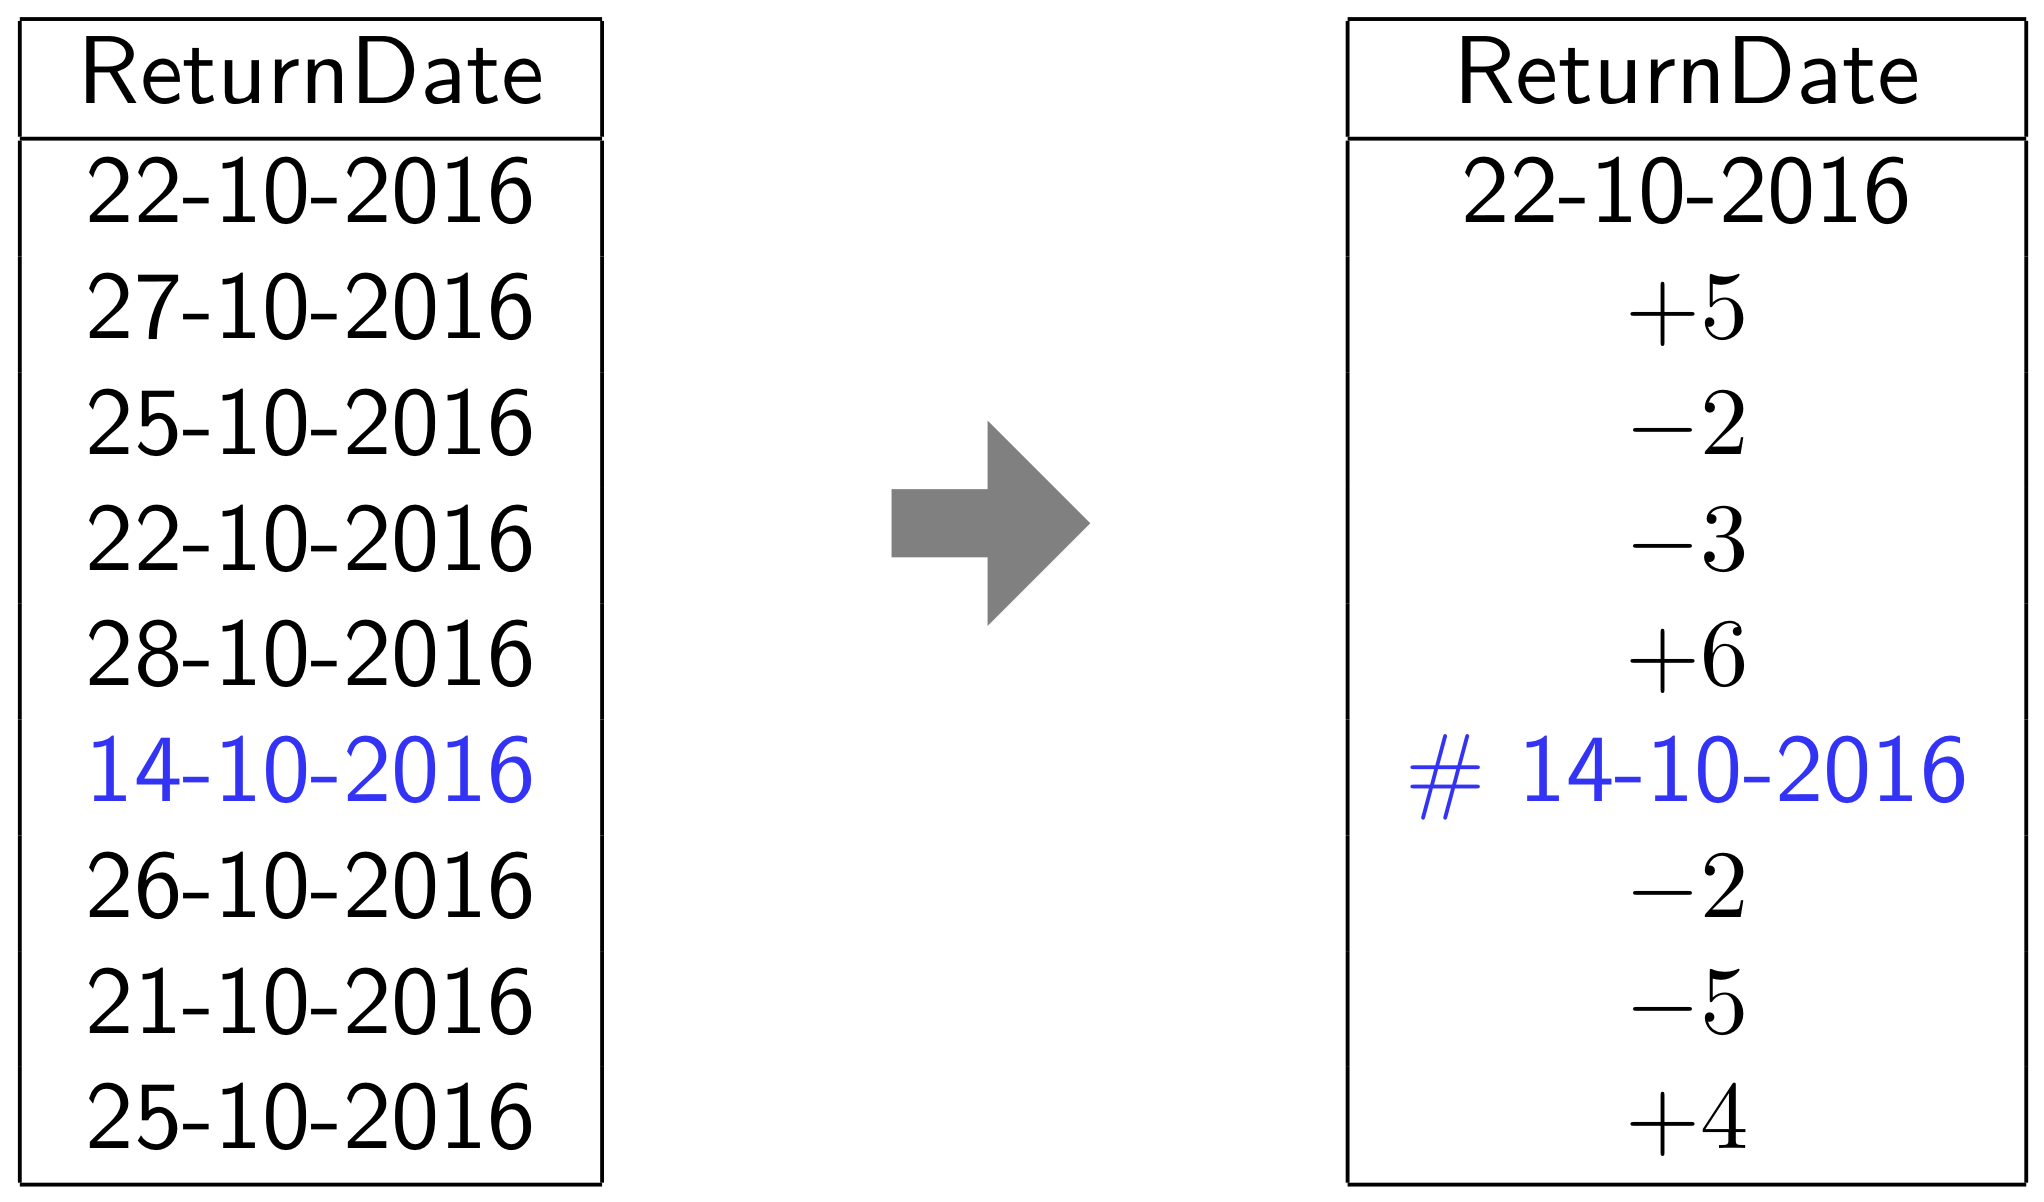
\includegraphics[width=0.60\linewidth]{images/AdvancedDataManagment/column_stores/differential_encoding.jpeg}
            \caption{Differential encoding example}
        \end{figure}
        
        \item \textbf{Disadvantages:}
        \begin{itemize}
            \item Extra runtime needed to compute the encoding
            \item Extra runtime needed to decode the data whenever we want to execute a query on them
        \end{itemize}
        \item Fortunately some queries can actually be executed on the compressed data so that no decompression step is needed. Like the following example:
        \vspace{0.3cm}
        We have that the ReaderID is encoded as a sequence as follows:
        \vspace{0.3cm}
        
        \centerline{((\textcolor{red}{205}, 1, 3), (\textcolor{orange}{207}, 4, 2), (\textcolor{red}{205}, 6, 1))}
        \vspace{0.3cm}
        Query: "How many books does each reader have?"
        \vspace{0.3cm}
        
        \centerline{SELECT ReaderID, COUNT(*) FROM BookLending GROUP BY ReaderID}
        \vspace{0.3cm}
        Now the column store does not have to decompress the column into the entire original column with 6 rows. It just returns (the sum of) the run-lengths for each ReaderID value.
        \begin{itemize}
            \item \textit{Reader 205} is 3 + 1 = 4
            \item \textit{Reader 207} is 2
        \end{itemize}
        
        \centerline{Result: \{(205, 4), (207, 2)\}}
    \end{itemize}
 \end{itemize}
 
\subsection{Null Suppression}
Sparse columns are columns that contain many NULL values. A more compact format of a sparse column can be achieved by \textbf{not storing these null values}, but some additional information is needed to distinguish the non-null columns from the null columns

\begin{itemize}
    \item \textbf{Position list:}
    \begin{itemize}
        \item List that stores only the non-null positions but discards any null values
        \item As metadata the total number of rows and the number of non-null positions are stored
    \end{itemize}
    
    
    %IMAGE
    
    
    \item \textbf{Position bit-string:}
    \begin{itemize}
        \item Bit-string for the column where non-null positions are set to 1 but null positions are set to 0
        \item Accompanied by a list of the non-null values in the order of their appearance in the column
    \end{itemize}

    %IAMGE

    \item \textbf{Position range:}
    \begin{itemize}
        \item If there are \textit{sequences of non-null values} in a column, the range of this sequence can be stored together with the list of values in the sequence
        \item As metadata the total number of rows and the number of non-null positions are stored
    \end{itemize}
\end{itemize}

\begin{tcolorbox}
These three encodings \textit{suppress nulls} and hence \textit{reduce the size of the data set}. However, internally, \textit{query evaluation} in the column store must be \textit{adapted to the null suppression} technique applied
\end{tcolorbox}

\section{Column striping}
The process of column striping decomposes a document into a set of columns:
\begin{itemize}
    \item One column for each unique path in the document
    \item For each unique path, the values coming from different documents are written to the same column in order to be able to answer analytical and aggregation queries over all documents efficiently
    \item  However we need some metadata to recombine an entire document as well as to be able to query it. These \textit{metadata} are called:
    \begin{itemize}
        \item \textit{Repetition level} to handle repetitions of paths and it denotes at which level in the path the last repetition occurred. Moreover it can range from \textbf{0} to the \textbf{path length}:
        \begin{itemize}
            \item \textbf{0:} no repetition has occurred so far
            \item \textbf{Path length:} denotes that the entire path occurred for the previous field
        \end{itemize}
        \item \textbf{Definition level} to handle non-existent paths of optional or repeated fields and it denotes the maximum level in the path for which a value exist. Only non-required fields are counted for the definition level
    \end{itemize}
\end{itemize}